%%%%%%%%%%%%%%%%%%%%%%%%%%%%%%%%%%%%%%%%%%%%%%%%%%%%%%%%%%
%%%%%%%%%%%%%%%%%%%%%%%%%%%%%%%%%%%%%%%%%%%%%%%%%%%%%%%%%%
\subsection{Technical details}
%%%%%%%%%%%%%%%%%%%%%%%%%%%%%%%%%%%%%%%%%%%%%%%%%%%%%%%%%%
%%%%%%%%%%%%%%%%%%%%%%%%%%%%%%%%%%%%%%%%%%%%%%%%%%%%%%%%%%


%%%%%%%%%%%%%%%%%%%%%%%%%%%%%%%%%%%%%%%%%%%%%%%%%%%%%%%%%%
\frame {\frametitle{I/O operations in Hadoop}
%%%%%%%%%%%%%%%%%%%%%%%%%%%%%%%%%%%%%%%%%%%%%%%%%%%%%%%%%%
  \begin{itemize}
  \item \textbf{Reading and writing data}
    \begin{itemize}
    \item From/to HDFS
    \item From/to local disk drives
    \item Across machines (inter-process communication)
    \end{itemize}

    \vspace{20pt}

  \item \textbf{Customized tools for large amounts of data}
    \begin{itemize}
    \item Hadoop does not use Java native classes
    \item Allows flexibility for dealing with custom data (e.g. binary)
    \end{itemize}

    \vspace{20pt}

  \item \textbf{What's next}
    \begin{itemize}
    \item Overview of what Hadoop offers
    \item For an in depth knowledge, use \cite{hadoop_book}
    \end{itemize}

  \end{itemize}

}

%%%%%%%%%%%%%%%%%%%%%%%%%%%%%%%%%%%%%%%%%%%%%%%%%%%%%%%%%%
%%%%%%%%%%%%%%%%%%%%%%%%%%%%%%%%%%%%%%%%%%%%%%%%%%%%%%%%%%
\subsection{Data Integrity}
%%%%%%%%%%%%%%%%%%%%%%%%%%%%%%%%%%%%%%%%%%%%%%%%%%%%%%%%%%
%%%%%%%%%%%%%%%%%%%%%%%%%%%%%%%%%%%%%%%%%%%%%%%%%%%%%%%%%%


%%%%%%%%%%%%%%%%%%%%%%%%%%%%%%%%%%%%%%%%%%%%%%%%%%%%%%%%%%
\frame {\frametitle{Data Integrity}
%%%%%%%%%%%%%%%%%%%%%%%%%%%%%%%%%%%%%%%%%%%%%%%%%%%%%%%%%%
  \begin{itemize}
  \item \textbf{Every I/O operation on disks or the network may
      corrupt data}
    \begin{itemize}
    \item Users expect data not to be corrupted during storage or
      processing
    \item Data integrity usually achieved with a simple \textbf{checksum} mechanism
    \end{itemize}

    \vspace{40pt}

  \item \textbf{HDFS transparently checksums all data during I/O}
    \begin{itemize}
    \item HDFS makes sure that storage overhead is roughly 1\%
    \item \texttt{DataNodes} are in charge of checksumming
      \begin{itemize}
      \item With replication, the last replica performs the check
      \item Checksums are timestamped and logged for
        {\color{red}statistics on disks}
      \end{itemize}
    \item Checksumming is also run periodically in a separate thread
      \begin{itemize}
      \item Note that thanks to replication, {\color{red}error
          correction} is possible in addition to detection
      \end{itemize}
    \end{itemize}


  \end{itemize}
}

%%%%%%%%%%%%%%%%%%%%%%%%%%%%%%%%%%%%%%%%%%%%%%%%%%%%%%%%%%
%%%%%%%%%%%%%%%%%%%%%%%%%%%%%%%%%%%%%%%%%%%%%%%%%%%%%%%%%%
\subsection{Data Compression}
%%%%%%%%%%%%%%%%%%%%%%%%%%%%%%%%%%%%%%%%%%%%%%%%%%%%%%%%%%
%%%%%%%%%%%%%%%%%%%%%%%%%%%%%%%%%%%%%%%%%%%%%%%%%%%%%%%%%%


%%%%%%%%%%%%%%%%%%%%%%%%%%%%%%%%%%%%%%%%%%%%%%%%%%%%%%%%%%
\frame {\frametitle{Compression}
%%%%%%%%%%%%%%%%%%%%%%%%%%%%%%%%%%%%%%%%%%%%%%%%%%%%%%%%%%
  \begin{itemize}
  \item \textbf{Why using compression}
    \begin{itemize}
    \item Reduce storage requirements
    \item Speed up data transfers (across the network or from disks)
    \end{itemize}

    \vspace{20pt}

  \item \textbf{Compression and Input Splits}
    \begin{itemize}
    \item IMPORTANT: use compression that supports
      {\color{red}splitting} (e.g. bzip2)
    \end{itemize}

    \vspace{20pt}

  \item \textbf{Splittable files, Example 1}
     \begin{itemize}
      \item Consider an uncompressed file of 1GB
      \item HDFS will split it in 16 blocks, 64MB each, to be
        processed by separate Mappers
      \end{itemize}
 \end{itemize}
}

%%%%%%%%%%%%%%%%%%%%%%%%%%%%%%%%%%%%%%%%%%%%%%%%%%%%%%%%%%
\frame {\frametitle{Compression}
%%%%%%%%%%%%%%%%%%%%%%%%%%%%%%%%%%%%%%%%%%%%%%%%%%%%%%%%%%
  \begin{itemize}
  \item \textbf{Unsplittable files, Example 2 (gzip)}
    \begin{itemize}
    \item Consider a compressed file of 1GB
    \item HDFS will split it in 16 blocks of 64MB each
    \item Creating an \texttt{InputSplit} for each block will not
      work, since it is not possible to read at an arbitrary point
    \end{itemize}

    \vspace{20pt}
    
  \item \textbf{What's the problem?}
    \begin{itemize}
    \item This forces MapReduce to treat the file as a
      {\color{red}single split}
    \item Then, a single Mapper is fired by the framework
    \item For this Mapper, only 1/16-th is local, the rest comes from
      the network
    \end{itemize}

    \vspace{20pt}

  \item \textbf{Which compression format to use?}
    \begin{itemize}
    \item Use bzip2
    \item Otherwise, use \texttt{SequenceFiles}
    \item See Chapter 4 \cite{hadoop_book}
    \end{itemize}

  \end{itemize} 
}

%%%%%%%%%%%%%%%%%%%%%%%%%%%%%%%%%%%%%%%%%%%%%%%%%%%%%%%%%%
%%%%%%%%%%%%%%%%%%%%%%%%%%%%%%%%%%%%%%%%%%%%%%%%%%%%%%%%%%
\subsection{Serialization}
%%%%%%%%%%%%%%%%%%%%%%%%%%%%%%%%%%%%%%%%%%%%%%%%%%%%%%%%%%
%%%%%%%%%%%%%%%%%%%%%%%%%%%%%%%%%%%%%%%%%%%%%%%%%%%%%%%%%%

%%%%%%%%%%%%%%%%%%%%%%%%%%%%%%%%%%%%%%%%%%%%%%%%%%%%%%%%%%
\frame {\frametitle{Serialization}
%%%%%%%%%%%%%%%%%%%%%%%%%%%%%%%%%%%%%%%%%%%%%%%%%%%%%%%%%%
  \begin{itemize}
  \item \textbf{Transforms structured objects into a byte stream}
    \begin{itemize}
    \item For transmission over the network: {\color{red}Hadoop uses RPC}
    \item For persistent storage on disks
    \end{itemize}

    \vspace{20pt}
    
  \item \textbf{Hadoop uses its own serialization format,
      \texttt{Writable}}
    \begin{itemize}
    \item Comparison of types is crucial (Shuffle and Sort phase):
      Hadoop provides a custom \texttt{RawComparator}, which avoids
      deserialization 
    \item Custom \texttt{Writable} for having full control on the
      binary representation of data
    \item Also ``external'' frameworks are allowed: enter \textbf{Avro}
    \end{itemize}

    \vspace{20pt}

  \item \textbf{Fixed-length or variable-length encoding?}
    \begin{itemize}
    \item Fixed-length: when the distribution of values is uniform
    \item Variable-length: when the distribution of values is not uniform
    \end{itemize}

  \end{itemize}
}

%%%%%%%%%%%%%%%%%%%%%%%%%%%%%%%%%%%%%%%%%%%%%%%%%%%%%%%%%%
%%%%%%%%%%%%%%%%%%%%%%%%%%%%%%%%%%%%%%%%%%%%%%%%%%%%%%%%%%
\subsection{Sequence Files}
%%%%%%%%%%%%%%%%%%%%%%%%%%%%%%%%%%%%%%%%%%%%%%%%%%%%%%%%%%
%%%%%%%%%%%%%%%%%%%%%%%%%%%%%%%%%%%%%%%%%%%%%%%%%%%%%%%%%%

%%%%%%%%%%%%%%%%%%%%%%%%%%%%%%%%%%%%%%%%%%%%%%%%%%%%%%%%%%
\frame {\frametitle{Sequence Files}
%%%%%%%%%%%%%%%%%%%%%%%%%%%%%%%%%%%%%%%%%%%%%%%%%%%%%%%%%%
  \begin{itemize}
  \item \textbf{Specialized data structure to hold custom input data}
    \begin{itemize}
    \item Using blobs of binaries is not efficient
    \end{itemize}

    \vspace{10pt}

  \item \textbf{\texttt{SequenceFiles}}
    \begin{itemize}
    \item Provide a persistent data structure for binary key-value
      pairs
    \item Also work well as containers for smaller files so that the
      framework is more happy (remember, better few large files than
      lots of small files)
    \item They come with the \texttt{sync()} method to introduce sync
      points to help managing \texttt{InputSplits} for MapReduce
    \end{itemize}

    \begin{center}
      \framebox{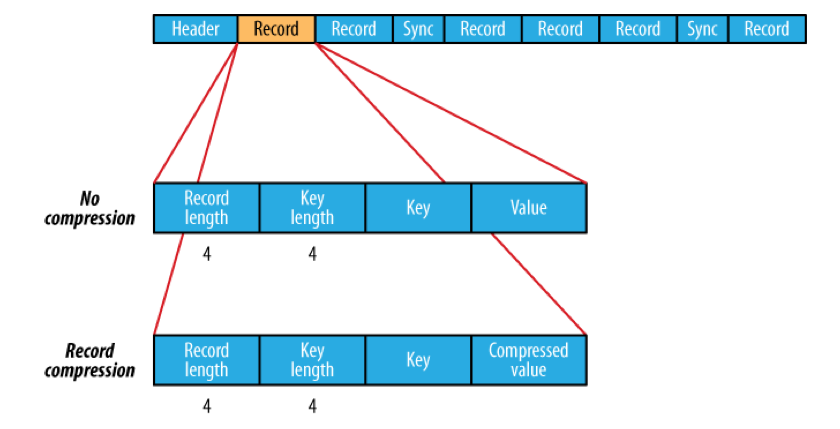
\includegraphics[scale=0.2]{./Figures/sequencefiles}}      
    \end{center}


  \end{itemize}
}

